\section{Development and Implementation}

Whilst the full source code is available in the appendix, the following section contains the most important parts of the code-base, highlighting the techniques used and technical solutions employed.

\subsection{Summary of techniques}
For handy reference, below is a table summarising the various techniques used in the codebase. \textbf{These are expanded upon in more detail below}.

{
	\renewcommand{\arraystretch}{1.5}
	\begin{table}[h!]
		\begin{center}
			\begin{tabularx}{1.0 \textwidth} {
					| >{\raggedright\arraybackslash}X 
					| >{\raggedright\arraybackslash}X
					| >{\raggedright\arraybackslash}X 
					|
				}
				\hline
				Source File & Technique & Purpose \\
				
				\hline
				include/data/atomic\_linked\_list.h & Thread-safe linked list (including linked list maintenance) from scratch and use of function callbacks & Provides data structure for inter-thread communication (see section 2.1) \\
				
				\hline
				include/data/tree.h and src/ui/file\_browser.cpp & Tree data structure and recursive navigation of filesystem & Used in file browsing to represent filesystem structure and allow the user to browse for audio files \\
				
				\hline
				src/data/merge-sort.cpp & Recursive merge-sort  algorithm implementation & To sort playlist files alphabetically \\
				
				\hline
				src/effects/fft.cpp & Cooley-Tukey Fast Fourier algorithm implementation & To aid in audio procession and visualisation \\
				
				\hline
				src/ui/audio\_visualiser.cpp & Uses FFT data & Renders audio visualisation \\
				
				\hline
				include/effects/audio\_effect.cpp & Polymorphic "audio effect" base class (inherited by children) - including use of hashmap & Manages common interface \\
				
				\hline
				include/effects/*property.h & Polymorphic "property" base class and associated children & Provides common interface for setting and getting properties of different types \\
				
				\hline
				src/effects/echo\_effect.cpp & Inheritance & Echo effect implementation \\
				
				\hline
				src/effects/equaliser\_effect.cpp &  Inheritance and use of Fourier algorithms & Audio equaliser implementation \\
				
				\hline
				src/effects/noise\_effect.cpp & Inheritance & Noise effect implementation \\
				
				\hline
				src/effects/volume\_effect.cpp & Inheritance & Volume effect implementation \\
				
				\hline
				Various files & Employing defensive programming patterns when reading and writing files to and from disk, as well as when modifying audio effects & Used with audio files , audio effects and playlists \\
				
				\hline
				src/io/audio\_stream.cpp, amongst others & Key program logic & Manages the audio playback loop, including processing and inter-thread communication. \\
				
				\hline
			\end{tabularx}
		\end{center}
	\end{table}
}

\pagebreak
\subsection{Atomic Linked List - \textit{include/data/atomic\_linked\_list.h}}
As discussed in section 2, the atomic linked list is a crucial component of the project, and was chosen as using a linked list means adding and removing elements can be done in constant time.  It makes use of generics (C++ "templates") to allow it to store any arbitrary data type. 

The full code is listed below, followed by explanations below of the most critical parts.

\inputminted[linenos]{c++}{../include/data/atomic_linked_list.h}

\paragraph{Mutexes} Whenever a caller accesses the data structure, the mutex is first locked. The relevant operation is then performed, and the mutex is then unlocked, freeing the data structure for future use (in this thread or otherwise). This can be seen in the functions Add, Remove, ForEach, SwapWithNext and Reset.

\paragraph{Generics} To make the data structure as flexible as possible, it is written to store a generic type "T". Note that we cannot store a variable of type T directly, but must rather store a pointer to each "T", as some types may be too big to store on the stack.

\paragraph{Callbacks} The data structure provides a "ForEach" method which takes a callback as an argument. This callback is invoked upon every node in the linked list, in order to allow for arbitrary operations to be formed on each element. This is used in \textit{src/io/audio\_stream.cpp} and \textit{src/ui/effects\_window.cpp} to iterate over each node. For example, in the \textit{AudioStream} class:
\begin{minted}{c++}
effects->ForEach([&](AudioEffect* effect) {
	effect->ApplyEffect(packet);
});
\end{minted}

\paragraph{Linked List Maintenance}  The head and tail pointers of affected nodes are updated when adding and removing a node (in the \textit{Add} and \textit{Remove} subroutines respectively), as well as when swapping two nodes (\textit{SwapWithPrevious} and \textit{SwapWithNext}). The head and tail pointers are then used when iterating over the list (for example in \textit{ForEach}), and when calling the destructor.


\pagebreak
\subsection{File Browser and Associated Tree - \textit{include/data/tree.h} and \textit{src/ui/file\_browser.cpp }}

The filesystem is inherently recursive - that is, folders may contain files, but also other folders, which may themselves contain other files and folders. In order to elegantly model this, I decided to use a recursive tree. This resulted in the ability to represent, in memory, the exact nature of the filesystem, allowing for the GUI display below:

\begin{figure}[h]
	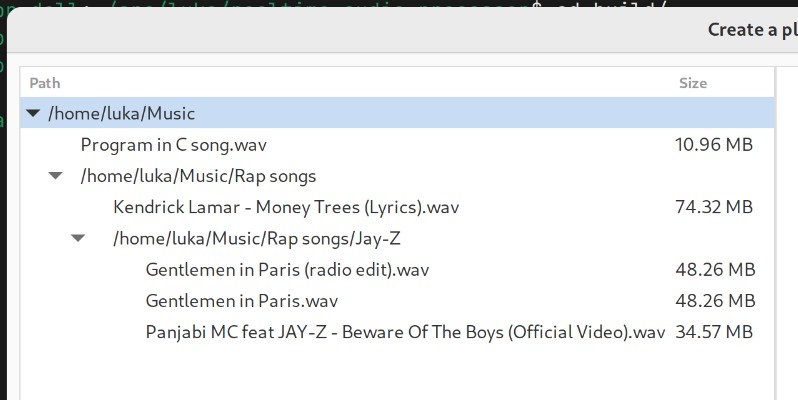
\includegraphics[width=13cm]{./file browser demo.png}
	\caption{Audio files are displayed in a graphical tree, backed by a tree in memory}
\end{figure}

\subsubsection{Tree data structure - \textit{include/data/tree.h}}
First, it was necessary to implement a tree data structure. Each node has a piece of data, followed by a list pointers to child nodes. Each child node may itself contain a piece of data, and a list of its own children.

As in C++ one must free explicit heap allocations manually,  recursion had to be used in the destructor. When the root node is destroyed, the following process occurs:
\begin{enumerate}
	\item C++ will call the destructor of the tree
	\item The tree iterates through all its children and calls their own respective destructors (line 16)
	\item This process repeats recursively until all children have deallocated their own children, and then finally themselves.
	\item Finally the root node deallocates itself.
\end{enumerate}
The full code is listed below.
\pagebreak
\inputminted[linenos]{c++}{../include/data/tree.h}

\pagebreak
\subsubsection{File Browser - \textit{src/ui/file\_browser.cpp}}
The file browser uses the tree data structure to store its files, and uses recursion to a greater extent. Below are the relevant parts of the code, followed by a description.

\inputminted[linenos, firstline=47, lastline=108]{c++}{../src/ui/file_browser.cpp}

\paragraph{The \textit{ScanDirectory} subroutine} This function is called on the root audio file directory (the user's Music folder). It creates a tree with a single node, containing the path to this directory. It then iterates through all the files and folders in the root directory. Files are added as children of the root node. If a directory is encountered instead, a tree for that directory is created by recursively calling \textit{ScanDIrectory} again, which is then added as a child to the existing tree. In this way, all files and folders contained within the root directory are added.  

\paragraph{The \textit{AddDirectory} subroutine} This subroutine is called once the tree containing all files and folders has already been created in \textit{ScanDirectory}. Each element is recursively added to a \textit{wxTreeListCtrl} (for the purposes of displaying the tree in the GUI) by first adding the directory itself, followed by the files contained within, then adding the sub-directories, which is done by recursively calling the function.

\pagebreak
\subsection{Merge Sort - \textit{src/data/merge\_sort.cpp}}
For ordering playlists alphabetically, a sorting  algorithm was needed. I decided to use a merge sort due to its low time complexity of \(O(N \log{N})\).
\inputminted[linenos]{c++}{../src/data/merge_sort.cpp}

\pagebreak
\subsection{Fourier Processing - \textit{src/effects/fft.cpp}}
This implements the pseudo-code produced in section 2.5, and hence uses recursion and the relevant Fourier maths, as well as linearising frequencies using the Bark scale. The relevant code is contained below.

\subsubsection{FFT Algorithm}
The Cooley-Tukey Fast Fourier Transform and corresponding Inverse Fast Fourier Transform are performed in the following function, using the pseudo-code written in Section 2. As such, it is recursive and manipulates each audio sample in the complex plane by manipulating its polar representation:
\inputminted[linenos, firstline=49, lastline=79]{c++}{../src/effects/fft.cpp}

\pagebreak
\subsubsection{Visualisation Algorithm}
As discussed in section 2.5, this transforms the data into a format easily plottable by the GUI code, and takes into account the non-linear scale of human hearing by using the Bark Scale and  a logarithmic scale for sound amplitude.

\paragraph{}
Converting from Hertz to the Bark scale is performed using the appropriate equation:
\inputminted[linenos, firstline=150, lastline=156]{c++}{../src/effects/fft.cpp}

\paragraph{}
The data is then converted into the desired "plottable format". To do this, two new structs are defined in the corresponding header file:
\inputminted[linenos, firstline=16, lastline=29]{c++}{../include/effects/fft.h}

\paragraph{}
Finally, the function known as \textit{convert\_fft\_to\_bar\_chart\_format} in the pseudo-code has been defined:
\inputminted[linenos, firstline=81, lastline=148]{c++}{../src/effects/fft.cpp}

\pagebreak
\subsubsection{Corresponding code to draw in GUI - \textit{src/ui/audio\_visualiser.cpp}}
Initially, results from the FFT were plotted straight to the screen. However, a key issue arose: audio changed so rapidly between frames that any visualisation was too flickery to be useful or readable.  To solve this, it was necessary to average the results of the FFT over multiple frames, so that changes in frequencies appeared more gradually. 

\paragraph{}
I also decided to colour the bars in the bar chart in accordance with their frequencies in order to increase the readability of the visualisation. It was also hoped that making the program more visually appealing would encourage more users to try it by capturing their attention. As I was, by default, displaying the full spectrum of audible frequencies, I wanted to intuitively communicate this using the full spectrum of colours. Modelling this using the typical RGB colour space was difficult. However luckily it is trivial using the HSV (hue-saturation-value) colour space, in which:
\begin{itemize}
	\item Hue represents the "base colour" (in essence the wavelength of light it corresponds to)
	\item Saturation represents the contrast of the colour
	\item Value represents the brightness of the colour
\end{itemize}
\inputminted[linenos, firstline=133, lastline=164]{c++}{../src/ui/audio_visualiser.cpp}

\paragraph{}
Each time a fixed buffer of audio is fed to the audio device (i.e. played to the speakers), the \textit{FeedAudio} subroutine is called, which performs a Fourier transform, adds it to the list of previous results for averaging, then triggers a GUI refresh.
\inputminted[linenos, firstline=15, lastline=44]{c++}{../src/ui/audio_visualiser.cpp}

\paragraph{}
When this GUI refresh occurs, it is finally time to draw the bar chart using the data stored in the class members:
\inputminted[linenos, firstline=67, lastline=131]{c++}{../src/ui/audio_visualiser.cpp}

\pagebreak
\subsection{Audio Effects and Properties}

\subsubsection{Base Audio Effect Class - \textit{include/effects/audio\_effect.h}}
The \textit{AudioEffect} base class has three key features:
\begin{enumerate}
	\item Provides a common interface for accessing "properties" (such as effect intensity). These properties are stored in a hashmap so that the names of the properties can be used as keys, and so that properties can be looked up with constant time complexity, which is important if any audio effects are added in the future that have a large number of properties to avoid wasting CPU cycles.
	\item Provides a common interface to identify the name of an effect in the GUI
	\item Provides a common interface to apply the effect to a "packet" of audio
\end{enumerate}

Here and elsewhere in the code, the project makes heavy use of OOP encapsulation. In this particular instance, external code remains unaware of each audio effect's particular property values or other member variables. Instead, audio effects can only be manipulated using the public interface defined. There is, however, an exception for the PropertiesWindow class due to performance concerns - this is discussed at length in the code's comments.    

\pagebreak
\inputminted[linenos]{c++}{../include/effects/audio_effect.h}

\pagebreak
\subsubsection{Property Base class - \textit{include/effects/property.h}}
\inputminted[linenos]{c++}{../include/effects/property.h}

\pagebreak
\subsubsection{IntegerProperty - \textit{include/effects/integer\_property.h}}
\inputminted[linenos]{c++}{../include/effects/integer_property.h}

\pagebreak
\subsubsection{FloatingPointProperty - \textit{include/effects/floating\_point\_property.h}}
\inputminted[linenos]{c++}{../include/effects/floating_point_property.h}


\pagebreak
\subsection{Implementation of Audio Effects - \textit{src/effects/*\_effect.cpp}}
Each audio effect was implemented using the flowcharts designed in section 2. Naturally, each audio effect class is a child of the base \textit{AudioEffect} class as discussed above.

\subsubsection{Echo Effect Header File - \textit{include/effects/echo\_effect.h}}
\inputminted[linenos]{c++}{../include/effects/echo_effect.h}
\pagebreak
\subsubsection{Echo Effect Source File - \textit{src/effects/echo\_effect.cpp}}
\inputminted[linenos]{c++}{../src/effects/echo_effect.cpp}

\pagebreak
\subsubsection{Equaliser Effect Header File - \textit{include/effects/equaliser\_effect.h}}
\inputminted[linenos]{c++}{../include/effects/equaliser_effect.h}
\pagebreak
\subsubsection{Equaliser Effect Source File - \textit{src/effects/equaliser\_effect.cpp}}
The equaliser effect is the only effect to manipulate audio in its frequency domain. As such, I encountered a variety of issues when implementing it:
\begin{itemize}
	\item One must be careful to not alter the phase of individual frequencies when adjusting the magnitudes - see EqualiserEffect::ModifyMagnitude
	\item Because audio "packets" are processed separately and then essentially "stitched together" when they are played in the real world by the user's speakers, it is crucial that there are no abrupt "jumps" in magnitude, as otherwise the speakers will not be able to physically move fast enough to accommodate this, causing crackling and significant noise. However, if one naively  processes audio packets without considering the adjacent packets, the discrete nature of the Discrete Fourier Transform will mean that the "boundaries" between packets will not perfectly align, resulting in this exact problem. The solution to this is discussed in detail within the code's comments, within the \textit{ApplyEffect} subroutine.
\end{itemize}
\inputminted[linenos]{c++}{../src/effects/equaliser_effect.cpp}

\pagebreak
\subsubsection{Noise Effect Header File - \textit{include/effects/noise\_effect.h}}
The noise effect uses a \textit{uniform real distribution}, so that all frequencies are equally affected. This is known as white noise, and mimics the backdrop of ambient sound. 
\inputminted[linenos]{c++}{../include/effects/noise_effect.h}
\pagebreak
\subsubsection{Noise Effect Source File - \textit{src/effects/noise\_effect.cpp}}
\inputminted[linenos]{c++}{../src/effects/noise_effect.cpp}

\pagebreak
\subsubsection{Volume Effect Header File - \textit{include/effects/volume\_effect.h}}
\inputminted[linenos]{c++}{../include/effects/volume_effect.h}
\pagebreak
\subsubsection{Volume Effect Source File - \textit{src/effects/volume\_effect.cpp}}
\inputminted[linenos]{c++}{../src/effects/volume_effect.cpp}


\pagebreak
\subsection{Defensive Programming}

\subsubsection{Reading Audio Files}
\paragraph{}
The AudioFile class provides an OOP interface for querying information about each file. Below is the definition in \textit{include/io/audio\_file.h}:
\inputminted[linenos]{c++}{../include/io/audio_file.h}

\paragraph{}
When loading an \textit{AudioFile} in the constructor, an exception is raised if an error occurs:
\inputminted[linenos, firstline=4, lastline=10]{c++}{../src/io/audio_file.cpp}

\paragraph{}
Then in \textit{src/ui/play\_window.cpp},  defensive programming is used to ensure the program does not behave incorrectly:
\pagebreak
\inputminted[linenos, firstline=303, lastline=348]{c++}{../src/ui/play_window.cpp}

\pagebreak
\subsubsection{Reading Playlists}
Recall that playlists are just text files where each line is a path to an audio file. Recall also that if an audio file is corrupt or does not exist, it will be caught later on when the audio file is read. However, it is still prudent to check the audio files do indeed exist when loading the playlist\footnote{
	This is purely for convenience. Imagine, for example, that a user has a very large playlist with hundreds of audio files. Rather than force them to listen to every single one to verify that they all exist on disk, let's check beforehand when the playlist is loaded too.
}. Below is the relevant code from \textit{src/io/playlist.cpp}:
\inputminted[linenos, firstline=25, lastline=55]{c++}{../src/io/playlist.cpp}

\paragraph{}
If this operation fails, the user will have an error message displayed in \textit{src/ui/start\_window.cpp}:
\inputminted[linenos, firstline=44, lastline=80]{c++}{../src/ui/start_window.cpp}

\pagebreak
\subsubsection{Saving Playlists}
Saving playlists is very straightforward as we know the files exist, given they have been selected within the program using the GUI. However we must still check the file can actually be saved. Below is the relevant code from \textit{src/io/playlist.cpp}:
\inputminted[linenos, firstline=25, lastline=55]{c++}{../src/io/playlist.cpp}

\paragraph{}
Naturally, we must also check the operation succeeded using a try-catch block in \textit{src/ui/playlist\_window.cpp}:
\inputminted[linenos, firstline=84, lastline=118]{c++}{../src/ui/playlist_window.cpp}

\pagebreak
\subsubsection{Defensive Programming with Audio Effects}
Whilst not strictly related to the saving and loading of audio files, defensive programming was also used in the effects window, where the user can remove effects or change the order in which they are applied. This was needed as:
\begin{enumerate}
	\item There is no guarantee that, when the user clicks the remove button, an audio effect was actually selected
	\item There should be no way for a user to move an effect already at the top of the list "even higher", and an audio effect at the bottom of the list "even lower".
\end{enumerate}
Below is the relevant code from \textit{src/ui/effects\_window.cpp}:
\inputminted[linenos, firstline=57, lastline=102]{c++}{../src/ui/effects_window.cpp}

\pagebreak
\subsection{Audio Playback Subroutines}
\paragraph{}
In section 2.2.5, an audio playback flowchart was designed, which formed the backbone of the project. In brief, it described a subroutine in which a buffer of audio was first fetched, processed by all active effects, then played by the system's speakers, all whilst being visualised on the GUI thread.

\subsubsection{Definition of Interfaces}
\paragraph{}
Naturally the management of this proved complicated, and so it was abstracted into the \textit{AudioStream} and \textit{AudioFile} class. Recall that UML class diagrams were designed for these in section 2.2.2.

\paragraph{}
The interface for the \textit{AudioFile} class was defined in \textit{include/io/audio\_file.h}:
\inputminted[linenos]{c++}{../include/io/audio_file.h}

\pagebreak
\paragraph{}
Next, the interface for the \textit{AudioStream} class was defined in \textit{include/io/audio\_stream.h}:
\inputminted[linenos]{c++}{../include/io/audio_stream.h}

\pagebreak
\subsubsection{Implementation of AudioStream Logic}
\paragraph{}
When an \textit{AudioStream} is created, it handles the creation of the SDL2 audio device, including verifying that the computer the software is running on supports the required settings. It also registers a callback so that, on a separate audio thread which will be created by SDL2, audio data can be sent to the operating system. This happens in the constructor of \textit{src/io/audio\_stream.cpp}:
 \inputminted[linenos, firstline=6, lastline=54]{c++}{../src/io/audio_stream.cpp}
 
 \pagebreak
 \paragraph{}
 When this audio callback occurs, five key steps occur:
 \begin{enumerate}
 	\item Buffers to the previous, current and next audio chunks from the \textit{AudioFile} are fetched
 	\item These are verified using the \textit{BufferIsInRange} function, as one can imagine not all three will be valid at the beginning or end of a file's playback.
 	\item The audio buffers are "resampled" if the playback speed has been modified (as the audio wave needs "squishing" or "stretching")
 	\item Next, the \textit{AudioEffect} instances stored in the "effects" \textit{AtomicLinkedList} are applied to the audio
 	\item Finally, the \textit{AudioStream} will call the \textit{on\_progress\_changed} callback, to notify the GUI that playback has advanced.
 \end{enumerate}
 
 \paragraph{}
 Below is the relevant code:
 \inputminted[linenos, firstline=68, lastline=177]{c++}{../src/io/audio_stream.cpp}
  
 \pagebreak
 \subsubsection{Communication with GUI thread}
 \paragraph{}
 When the AudioStream is created in \textit{src/ui/play\_window.cpp}, its callback is set. Care is taken to enqueue the work needed to the GUI thread using a custom-defined event:
 \inputminted[linenos, firstline=341, lastline=345]{c++}{../src/ui/play_window.cpp}
 
 \paragraph{}
 The \textit{AudioStreamUpdatedEvent} is a derived from the wxEvent class, and contains the needed data for the updating of the GUI. The code is contained under \textit{include/ui/custom\_events.h}:
 \inputminted[linenos]{c++}{../include/ui/custom_events.h}
 
 \pagebreak
 \paragraph{}
Hence the \textit{AudioStream} callback arrives at the following code in \textit{src/ui/play\_window.cpp}, in which the GUI is updated. Recall that the contents of the FeedAudio subroutine has already been covered in section 3.5.3.
\inputminted[linenos, firstline=350, lastline=362]{c++}{../src/ui/play_window.cpp}
 